\documentclass[12pt,a4paper]{article}
\usepackage[utf8]{inputenc}
\usepackage[english]{babel}
\usepackage[T1]{fontenc}
\usepackage{amsmath}
\usepackage{amsfonts}
\usepackage{amssymb}
\usepackage{graphicx}
\usepackage{siunitx}
\usepackage{float}
\usepackage[left=2cm,right=2cm,top=2cm,bottom=2cm]{geometry}
\author{Gerald}

\begin{document}
\sisetup{separate-uncertainty = true}
	\setlength{\parindent}{0pt} 
	\begin{center}
		{\LARGE Experiment protocoll}\\
		\begin{large}
			for the solid state lab course\\[0.4cm]
			at RWTH Aachen\\
			II. Physikalisches Institut A\\[5.5cm]
			\Large\textbf{\textsl{Superconductivity and SQUID}}\\[5.5cm]
			\normalsize\textit{authored\\by}\\[0.4cm]
			\large{Moritz Berger (355244)\\Gerald Kolter (355005)}\\[2cm]
			\large \textbf{Summer term 2019}
		\end{large}
	\end{center}
	\newpage
	
	\tableofcontents
	\newpage

\section{Introduction}
\section{Goal of the Experiment}
\section{Setup}
\section{Measurement}
\section{Data}
\section{Results and Discussion}
\section{Conclusion}


%\begin{figure}
%\centering
%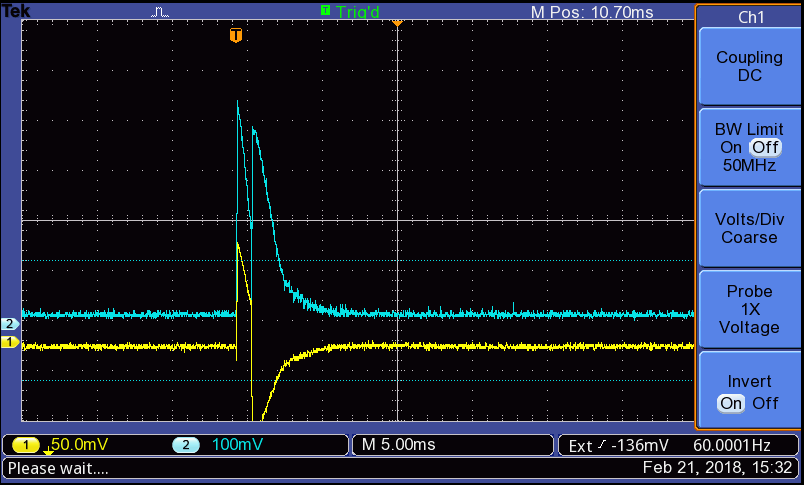
\includegraphics[scale=0.8]{Bilder/F0003TEK.PNG}
%\caption{Ergebnis einer einzelnen Messung zur Bestimmung von T1. Die blaue Kurve zeigt das zu untersuchende Signal.}
%\label{fig:MessungT1_Beispiel}
%\end{figure}



%\begin{table}
%\centering
%\begin{tabular}{|c|c|c|}
%\hline 
%Pulshöhe [mV] & FID-Höhe [mV] & $\tau$ [ms] \\ 
%\hline 
%428 $\pm$ 4 & -376 $\pm$ 4 & 0.918 $\pm$ 0.042 \\ 
%\hline 
%432 $\pm$ 4 & -360 $\pm$ 4 & 1.800 $\pm$ 0.042 \\ 
%\hline 
%432 $\pm$ 4 & -336 $\pm$ 4 & 2.700 $\pm$ 0.042 \\ 
%\hline 
%452 $\pm$ 4 & -308 $\pm$ 4 & 3.618 $\pm$ 0.042 \\ 
%\hline 
%452 $\pm$ 4 & -276 $\pm$ 4 & 4.554 $\pm$ 0.042 \\ 
%\hline 
%432 $\pm$ 4 & -248 $\pm$ 4 & 5.436 $\pm$ 0.042 \\ 
%\hline 
%440 $\pm$ 4 & -216 $\pm$ 4 & 6.300 $\pm$ 0.042 \\ 
%\hline 
%428 $\pm$ 4 & -184 $\pm$ 4 & 7.290 $\pm$ 0.042 \\ 
%\hline 
%440 $\pm$ 4 & -156 $\pm$ 4 & 8.154 $\pm$ 0.042 \\ 
%\hline 
%436 $\pm$ 4 & -116 $\pm$ 4 & 9.036 $\pm$ 0.042 \\ 
%\hline 
%436 $\pm$ 4 & -104 $\pm$ 4 & 9.954 $\pm$ 0.042 \\ 
%\hline 
%432 $\pm$ 4 & -72 $\pm$ 4 & 10.854 $\pm$ 0.042 \\ 
%\hline 
%424 $\pm$ 4 & -52 $\pm$ 4 & 11.862 $\pm$ 0.042 \\ 
%\end{tabular} 
%\caption{Messwerte der Höhen des $\pi /2$-Pulses und des FID s beim Durchfahren von $\tau$ zur Bestimmung von T1.}
%\label{tab:T1_Daten}
%\end{table}




\end{document}